\chapter{Analysis methods for the fully hadronic VBS aQGC search}
\label{chap:analysismethods}

This chapter describes the machine learning methods developed to maximise sensitivity to anomalous quartic gauge couplings in the fully hadronic VBS analysis. The analysis targets the electroweak production of two vector bosons in association with two forward jets, $pp \to VVjj$, where both bosons decay hadronically. The signal topology consists of two large-$R$ UFO jets from the boosted vector boson decays and two small-$R$ forward PFlow tagging jets. The dominant background is QCD multijet production, which exceeds the EWK signal cross section by approximately eight orders of magnitude in the analysis phase space, making dedicated event classification essential.

Events are selected through a sequential pipeline. First, a pre-selection is applied requiring at least two large-$R$ jets, a single large-$R$ jet trigger, a leading jet $p_T > 560$~GeV and a dijet invariant mass $m_{JJ} > 1.3$~TeV. The pre-selection criteria are summarised in Table~\ref{tab:analysis_selection}.

\begin{table}[htbp]
  \centering
  \caption{Pre-selection applied in the analysis.}
  \label{tab:analysis_selection}
  \begin{tabular}{|c|c|}
    \hline
    \textbf{Stage} & \textbf{Requirements} \\
    \hline
    Pre-selection & $\geq 2$ large-$R$ jets \\
                  & Leading signal jet $p_T > 560$~GeV \\
                  & Sub-leading signal jet $p_T > 200$~GeV \\
                  & $m_{JJ} > 1.3$~TeV \\
    \hline
  \end{tabular}
\end{table}

The VBF-RNN tagger, described in detail in Section~\ref{sec:vbfrnn}, assigns a score reflecting the probability that an event originates from a VBS topology based on the kinematics of the forward tagging jets and signal jets. The VBF-RNN tagger is trained and evaluated directly on the pre-selected sample without any additional boson tagger requirement. A further training selection, which moves the phase space close to the analysis signal region and is described in Section~\ref{sec:mldiscriminant}, is applied when training and evaluating the MLP-based aQGC discriminant.

The full dataset corresponds to the full Run~2 MC simulation at $\sqrt{s} = 13$~TeV with an integrated luminosity of $140~\text{fb}^{-1}$. Signal and electroweak background events are generated with \texttt{MadGraph5\_aMC@NLO}~\cite{Alwall:2014MG5} using the Éboli dimension-eight basis~\cite{Eboli_2016}, with only the pure-EFT quadratic contribution included. Parton showering and hadronisation are simulated with \texttt{Pythia 8}~\cite{Sjostrand:2015Pythia8}, and the detector response is modelled with \texttt{Geant4}~\cite{Agostinelli:2003Geant4} in the full ATLAS simulation chain. The background composition in the signal region is dominated by QCD dijet production ($\sim\!96\%$), with subdominant contributions from $V$+jets ($\sim\!3\%$), $t\bar{t}$ ($\sim\!1\%$), QCD diboson and electroweak $VV$+$jj$ production. The signal samples consist of aQGC EFT operators from the scalar ($S$), mixed ($M$) and tensor ($T$) families.

The chapter is organised as follows. Section~\ref{sec:vbfrnn} describes the VBF-RNN tagger and its adaptation for the fully hadronic VBS channel. Section~\ref{sec:mldiscriminant} presents the MLP-based aQGC discriminant, covering the binary and multiclass classifiers and the sensitivity results.

\section{Vector boson scattering topology identification}
\label{sec:vbfrnn}

The physical process targeted by this analysis is the electroweak production of two vector bosons in association with two jets, $pp \to VVjj$~(EWK). This inclusive EWK process contains both VBS and non-VBS contributions, illustrated in Figure~\ref{fig:ewk_diagrams}: the VBS subprocess (Figure~\ref{fig:vbs_ewk}) proceeds through a genuine $VV \to VV$ scattering vertex and exhibits the characteristic forward-jet topology that distinguishes it from the non-VBS EWK diagrams (Figure~\ref{fig:novbs_ewk}), in which the vector bosons are radiated from the quark lines and contribute to the same $VVjj$ final state. Extracting the VBS component from the broader EWK $VVjj$ production is therefore a necessary step before searching for anomalous couplings.

\begin{figure}[htbp]
\centering
\begin{subfigure}[b]{0.40\textwidth}
\centering
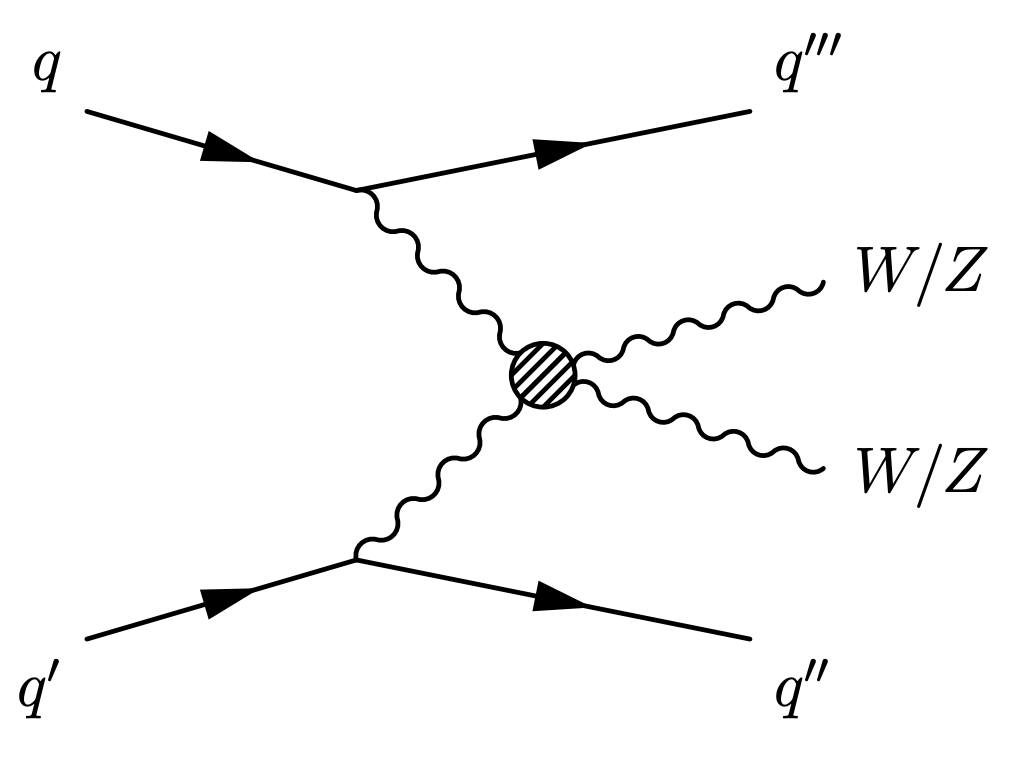
\includegraphics[width=\textwidth]{figures/vbs_ewk.png}
\caption{}
\label{fig:vbs_ewk}
\end{subfigure}
\hfill
\begin{subfigure}[b]{0.40\textwidth}
\centering
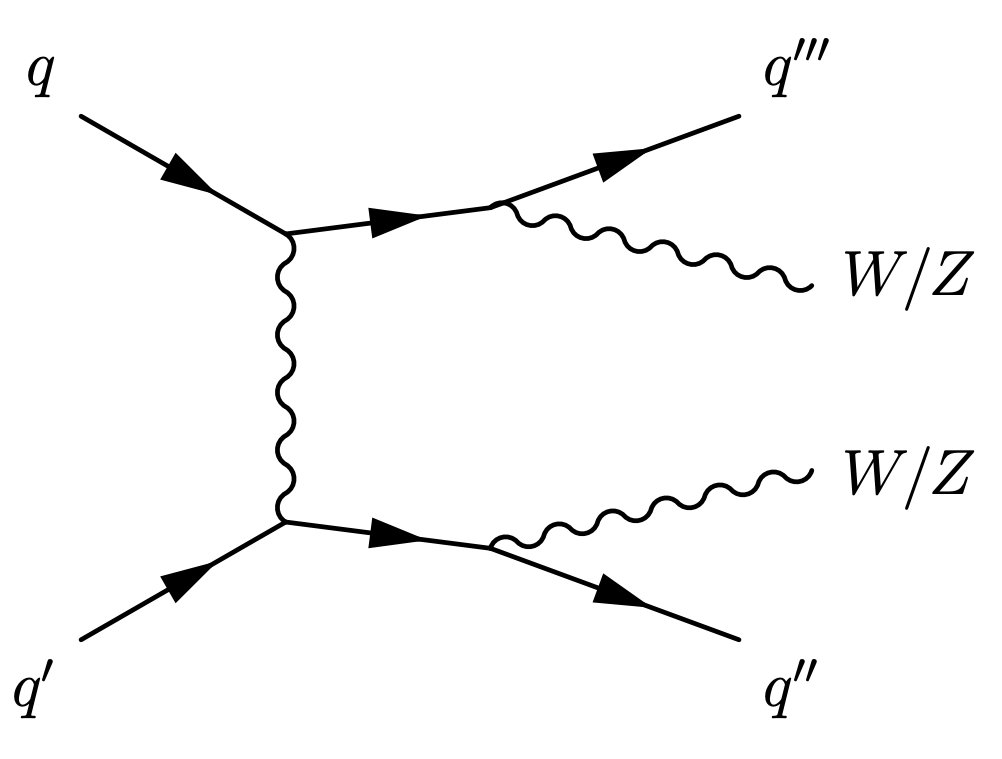
\includegraphics[width=\textwidth]{figures/novbs_ewk.png}
\caption{}
\label{fig:novbs_ewk}
\end{subfigure}
\caption{Representative diagrams for the electroweak production of two vector bosons in association with two jets, $pp \to VVjj$~(EWK). (a) The VBS subprocess, in which the two incoming quarks each radiate a vector boson that subsequently scatter, $VV \to VV$, producing the two forward tagging quarks $q''$ and $q'''$ and the two final-state bosons. (b) A non-VBS EWK diagram contributing to the same final state, in which the vector bosons are radiated from the quark lines without a genuine boson scattering vertex.}
\label{fig:ewk_diagrams}
\end{figure}

The VBF-RNN tagger was originally developed to identify the characteristic forward-jet topology of vector boson fusion and vector boson scattering processes and has been deployed in previous ATLAS measurements including the semi-leptonic VBS analysis~\cite{Antonio_VBFRNN_2023}. In this analysis the tagger is adapted and re-optimised for the fully hadronic VBS channel, where both the tagging jets and the signal jets from the hadronically decaying bosons are available as inputs.

The classification task is formulated as a supervised binary problem: each event is assigned a label $y = 1$ if it originates from a VBS process and $y = 0$ if it originates from a non-VBS EWK process. To define these labels at the truth level, jets in the training sample are matched to their underlying hard-scatter particles. Boson matching is performed using a $\Delta R$ criterion of $\Delta R < 1.0$ for large-$R$ jets and $\Delta R < 0.4$ for small-$R$ jets. Jets are identified by a subtraction strategy: a jet is labelled as a VBS tagging jet if it is not boson-matched, not gluon-initiated and not consistent with pileup.

Three versions of the tagger are developed for this analysis, differing in the set of jets provided as input and the training sample used and are summarised in Table~\ref{tab:vbfrnn_versions}.

\begin{table}[htbp]
  \centering
  \caption{Summary of the three VBF-RNN versions developed for this analysis. All versions use jet four-momenta $(p_T, \eta, \phi, E)$ as input features.}
  \label{tab:vbfrnn_versions}
  \begin{tabular}{|c|c|c|}
    \hline
    \textbf{Version} & \textbf{Input jets} & \textbf{Training task} \\
    \hline
    v1 & Up to 4 tagging jets            & Resonance VBF vs.\ ggF \\
    v2 & Up to 4 tagging jets            & VBS vs.\ non-VBS (EWK) \\
    v3 & Up to 6 jets (tagging + signal) & VBS vs.\ non-VBS (EWK) \\
    \hline
  \end{tabular}
\end{table}

Version~1 corresponds to the configuration used in earlier analyses~\cite{Antonio_VBFRNN_2023}, trained to separate a heavy scalar resonance produced through vector boson fusion from the same resonance produced through gluon fusion (here $H\to q\bar{q}q\bar{q}$ at $m_H = 3$~TeV), using only the potential tagging jets. Because its training signal is a spin-0 resonance whose decay bosons are predominantly longitudinally polarised, version~1 effectively learns a longitudinal, scalar-like topology, a point that becomes important when its response to the aQGC operator families is examined in Chapter~\ref{chap:vbfrnn_results}. This version provides a useful baseline and demonstrates that the topological characteristics of VBF-like events are captured by the tagging-jet kinematics alone. Version~2 retrains the same four-jet architecture directly on the VBS versus non-VBS (EWK) classification task relevant to this analysis. Version~3 extends the input to six jets by including the two large-$R$ signal jets alongside the tagging jets, giving the network access to the full reconstructed final state.

The four tagging jets constrain only the production side of the event, but the VBS and non-VBS EWK subprocesses also differ in the diboson system they produce. The genuine $VV\to VV$ scattering of the VBS subprocess yields a harder, higher-mass central diboson pair than the radiative non-VBS EWK topologies that share the same final state. Figure~\ref{fig:vbfrnn_sigjet} exposes this residual difference through the dijet invariant mass of the two large-$R$ signal jets, which retains discriminating power between the two classes that the tagging jets do not capture and which is largely statistically independent of the production-side information. The residual difference motivates the six-jet configuration of version~3. The separation is shown for the $WZjj\to4q$ channel, but it originates in the diboson scattering kinematics rather than in the specific boson decay and is therefore representative of all diboson channels. The combined-channel performance reported in Chapter~\ref{chap:vbfrnn_results} confirms that the gain carries over to the inclusive sample.

\begin{figure}[htbp]
\centering
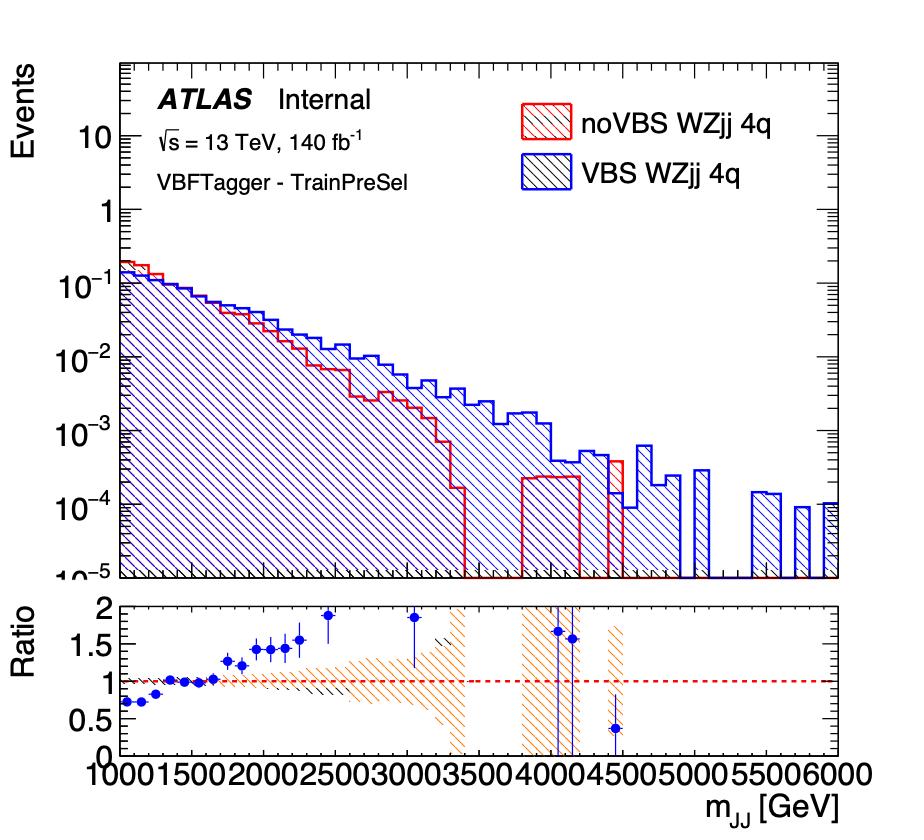
\includegraphics[width=0.6\textwidth]{figures/vbfrnn_sigjet_mjj.png}
\caption{Distribution of the dijet invariant mass of the two large-$R$ signal jets, for VBS (blue) and non-VBS EWK (red) $VV+jj$ events. The difference between the two distributions, shown by the ratio panel, demonstrates the additional discriminating information that motivates including the signal jets in version~3 of the tagger.}
\label{fig:vbfrnn_sigjet}
\end{figure}

\subsection{Input representation}

For each jet, the observables $(p_T,\,\eta,\,\phi,\,E)$ are used as input features, forming a tensor $\mathbf{X} \in \mathbb{R}^{T \times 4}$ for a sequence of $T$ jets ordered by decreasing transverse momentum. Events with fewer than $T$ jets are zero-padded to the fixed sequence length and the padding is masked during the forward pass so that padded steps do not contribute to the hidden-state evolution, as described in Chapter~\ref{chap:ml}.

The jet four-vector representation is a deliberate design choice. Jet constituents (tracks, calorimeter clusters or PFlow/UFO objects) carry richer substructure information and would, in principle, improve a stand-alone classifier. They, however, require a dedicated calibration chain and a fixed operating point for every downstream analysis that uses them, since the constituent-level response is process-dependent and is corrected through working-point-specific scale factors. The VBF-RNN is explicitly designed to be reused as an input feature by further ML models downstream in the analysis, in particular the aQGC discriminant of Section~\ref{sec:mldiscriminant}. Tying the upstream tagger to a constituent-level calibration and a fixed working point would propagate those choices into every downstream model and would force a re-calibration whenever the operating point is changed. Restricting the input to the calibrated jet four-vector avoids both issues: the inputs are already calibrated at jet level by the standard ATLAS jet calibration chain, no tagger-specific working point is required, and the resulting score can be passed unchanged to any downstream model.

\subsection{Architecture and training}

The network consists of two stacked LSTM layers. The first layer processes the jet sequence and produces an intermediate hidden-state sequence encoding inter-jet correlations. The second layer refines this representation and returns the hidden state at the final time step, $\mathbf{h}_T \in \mathbb{R}^d$, which constitutes a fixed-length summary of the entire event. This vector is passed to a dense output layer with sigmoid activation, yielding a scalar score $s \in [0,1]$ interpreted as the posterior probability $P(y=1 \mid \mathbf{X})$ that the event originates from a VBS process. The architecture is illustrated in Figure~\ref{fig:vbfrnn}.

\begin{figure}[htbp]
\centering
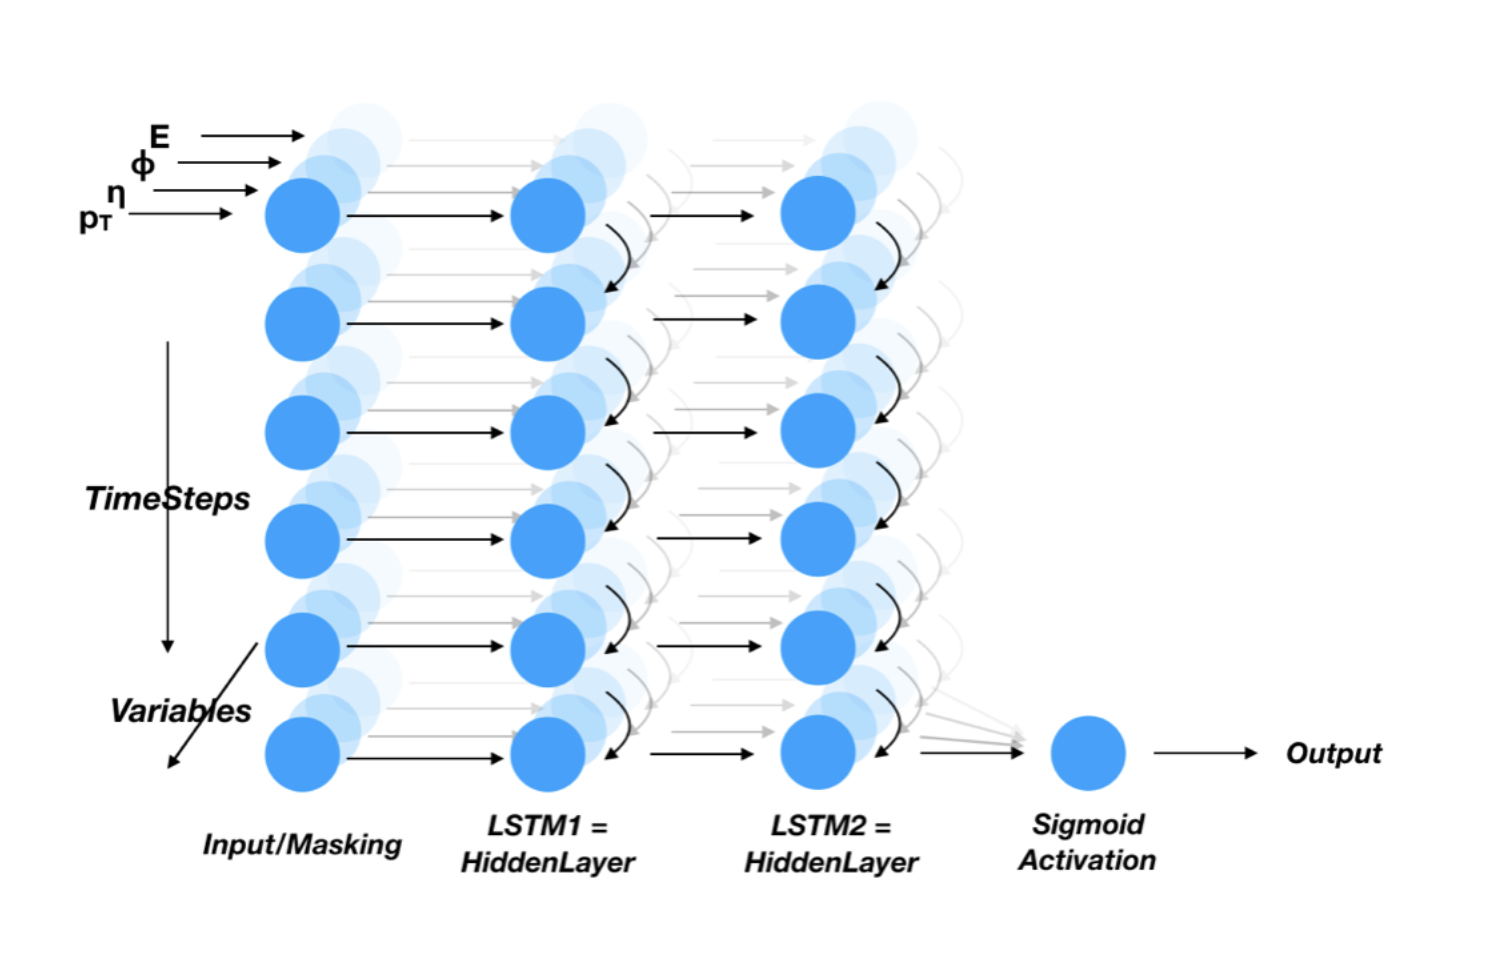
\includegraphics[scale=0.45]{figures/VBFRNN.png}
\caption{Illustration of the VBF-RNN architecture \cite{Antonio_VBFRNN_2023}. The input sequence of jet four-vectors is processed by two stacked LSTM layers and the final hidden state is passed to a sigmoid output node.}
\label{fig:vbfrnn}
\end{figure}

Each LSTM layer has a hidden dimension of $25$, with a dropout and recurrent dropout of $0.3$ applied for regularisation. The network is trained for up to $200$ epochs by minimising a per-event-weighted binary cross-entropy loss over mini-batches of labelled Monte Carlo events, with the Monte Carlo event weight used as the per-example weight so that the optimisation reflects the physical sample composition. The available dataset is partitioned into statistically independent training and validation samples in an $80/20$ split, only the training sample contributes to parameter updates, while the validation sample is used to monitor performance and select the final network configuration. The hyperparameters, common to all three versions, are summarised in Table~\ref{tab:rnn_hyperparams}. The VBF-RNN score is used both as a pre-selection requirement to enrich the sample in VBS-topology events and as one of the input features to the aQGC discriminant described in Section~\ref{sec:mldiscriminant}.

\begin{table}[htbp]
  \centering
  \caption{Architecture and training hyperparameters of the VBF-RNN, common to all three versions. The number of input jets is the only structural difference: four for versions~1 and~2, six for version~3.}
  \label{tab:rnn_hyperparams}
  \begin{tabular}{|c|c|}
    \hline
    \textbf{Hyperparameter} & \textbf{Value} \\
    \hline
    Stacked LSTM layers          & 2 \\
    Dimension per hidden layer   & 25 \\
    Dropout                      & 0.3 \\
    Recurrent dropout            & 0.3 \\
    Output activation            & sigmoid \\
    Loss                         & binary cross-entropy \\
    Training epochs              & 200 \\
    Train\,/\,validation split   & 80\,/\,20 \\
    Input features per jet       & 4 ($p_T,\eta,\phi,E$) \\
    Maximum input jets                   & Up to 4 (v1, v2) / Up to 6 (v3) \\
    \hline
  \end{tabular}
\end{table}

\subsection{Alternative transformer architecture}

As an alternative to the recurrent architecture, a transformer encoder was also trained on the identical six-jet input and VBS versus non-VBS EWK target as version~3. Instead of propagating information sequentially, it computes pairwise interactions between all input jets simultaneously through the self-attention mechanism described in Chapter~\ref{chap:ml}. The configuration, summarised in Table~\ref{tab:transformer_hyperparams}, comprises four stacked self-attention blocks with four heads each, a $64$-dimensional jet embedding and a two-layer classifier head, it is a substantially higher-capacity model than the two-layer, width-$25$ LSTM of the VBF-RNN. Its performance relative to version~3 is evaluated in Chapter~\ref{chap:vbfrnn_results}.

\begin{table}[htbp]
  \centering
  \caption{Architecture and training hyperparameters of the transformer encoder, trained on the same six-jet input and VBS versus non-VBS EWK target as version~3.}
  \label{tab:transformer_hyperparams}
  \begin{tabular}{|c|c|}
    \hline
    \textbf{Hyperparameter} & \textbf{Value} \\
    \hline
    Self-attention blocks                       & 4 \\
    Attention heads                             & 4 \\
    Head size                                   & 32 \\
    Jet embedding dimension                     & 64 \\
    Embedding MLP units                         & [64, 64] \\
    Feed-forward dimension                      & 128 \\
    Classifier MLP units                        & [128, 64] \\
    Dropout (embedding / block / classifier)    & 0.15 / 0.25 / 0.20 \\
    Output activation                           & sigmoid \\
    Training epochs                             & 200 \\
    Input features per jet                      & 4 ($p_T,\eta,\phi,E$) \\
    Maximum input jets                          & Up to 6 \\
    \hline
  \end{tabular}
\end{table}

\section{Machine-learning aQGC discriminant}
\label{sec:mldiscriminant}

While the VBF-RNN identifies the characteristic topology of VBS events, the primary goal of this analysis is to maximise sensitivity to anomalous quartic gauge couplings. The discriminating information between aQGC signal and background is distributed across several event-level observables, motivating the use of an MLP to combine them optimally into a single discriminant.

To define a training selection that moves the phase space close to the analysis signal region, a dedicated boson tagger is applied to the large-$R$ jets. The DisCoJet tagger is an ATLAS machine learning based classifier trained to identify large-$R$ jets consistent with hadronic $W$ or $Z$ boson decays using jet substructure observables. A key property of DisCoJet is that it is explicitly decorrelated from the jet mass, achieved by applying the distance correlation (DisCo) technique described in Section~\ref{sec:disco}~\cite{Kasieczka:2020DisCo} during training to minimise the statistical dependence between the tagger score and the jet mass. This decorrelation ensures that the tagger score does not sculpt the jet mass distribution, preserving the latter as a useful observable in the analysis.

A training selection is defined to bring the phase space close to the analysis signal region without yet defining it exactly. It requires a VBF-RNN v3 score above 0.3 and a DisCoJet score above 0.65 for both large-$R$ jets, as summarised in Table~\ref{tab:mlp_selection}. The MLP-based discriminant is trained and evaluated within this selection.

\begin{table}[htbp]
  \centering
  \caption{Training selection applied for MLP training and evaluation, it moves the phase space close to the analysis signal region.}
  \label{tab:mlp_selection}
  \begin{tabular}{|c|c|}
    \hline
    \textbf{Stage} & \textbf{Requirements} \\
    \hline
    Training selection & VBF-RNN v3 score $> 0.3$ \\
                            & DisCoJet score $> 0.65$ for both large-$R$ jets \\
    \hline
  \end{tabular}
\end{table}

\subsection{Input features and training samples}

The MLP takes twelve event-level features as input: the transverse momentum, pseudorapidity, azimuthal angle and invariant mass of each of the two leading large-$R$ signal jets, the VBF-RNN score from version~3 of the tagger and three multiplicity variables: the number of tagging jets provided to the RNN, the total number of small-$R$ jets and the number of large-$R$ jets. All features are standardised to zero mean and unit variance prior to training, as discussed in Chapter~\ref{chap:ml}. Normalised distributions of the input variables for representative S0, M0 and T0 aQGC signal samples and the composite background are shown in Figures~\ref{fig:input_distributions} and~\ref{fig:input_distributions_extra}.

\begin{figure}[htbp]
\centering
\begin{subfigure}[b]{0.4\textwidth}
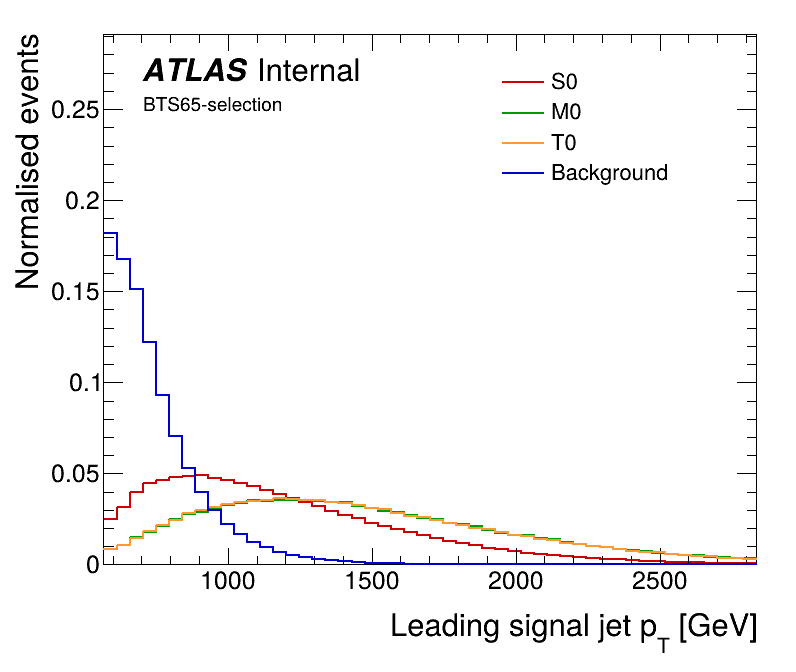
\includegraphics[width=\textwidth]{figures/SigJet1_pT_NOSYS.png}
\end{subfigure}
\hfill
\begin{subfigure}[b]{0.4\textwidth}
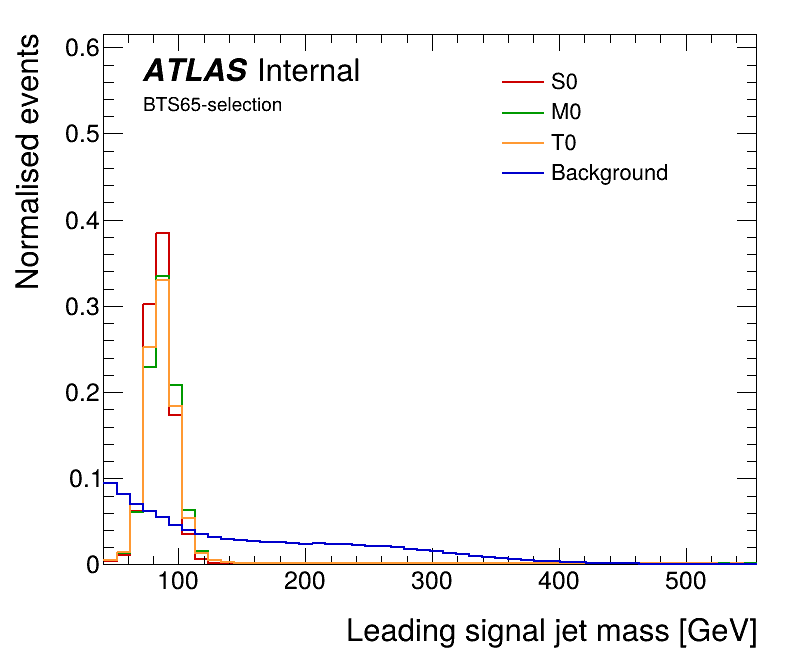
\includegraphics[width=\textwidth]{figures/SigJet1_M_NOSYS.png}
\end{subfigure}

\medskip

\begin{subfigure}[b]{0.4\textwidth}
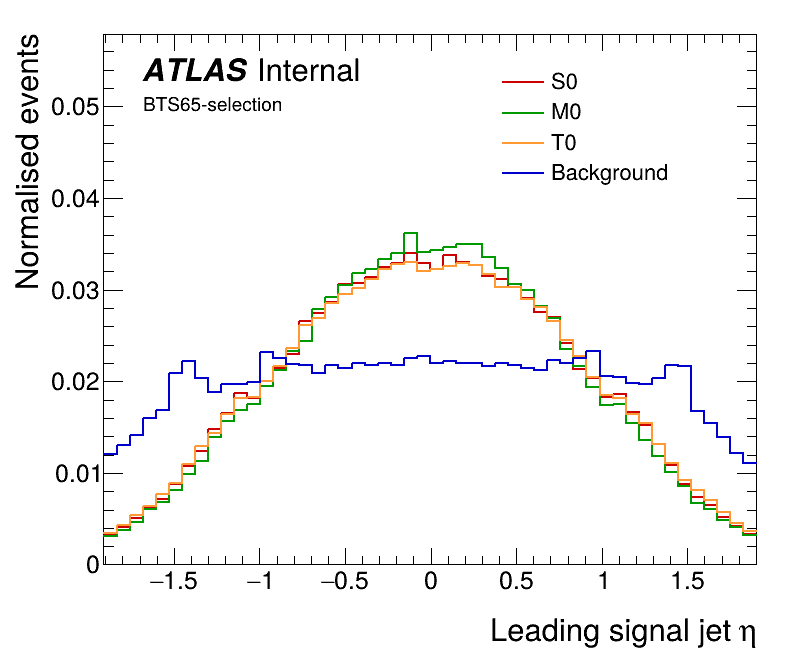
\includegraphics[width=\textwidth]{figures/SigJet1_eta_NOSYS.png}
\end{subfigure}
\hfill
\begin{subfigure}[b]{0.4\textwidth}
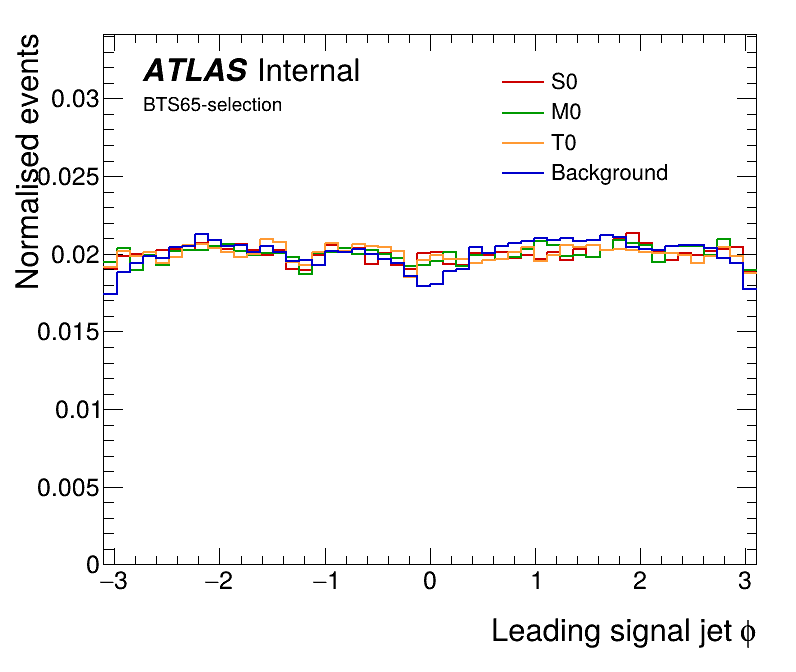
\includegraphics[width=\textwidth]{figures/SigJet1_phi_NOSYS.png}
\end{subfigure}

\medskip

\begin{subfigure}[b]{0.4\textwidth}
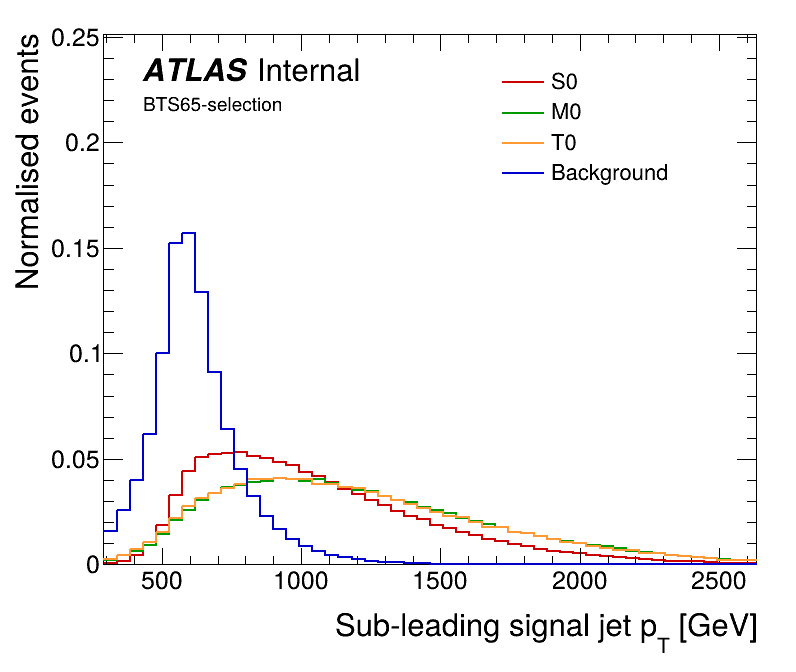
\includegraphics[width=\textwidth]{figures/SigJet2_pT_NOSYS.png}
\end{subfigure}
\hfill
\begin{subfigure}[b]{0.4\textwidth}
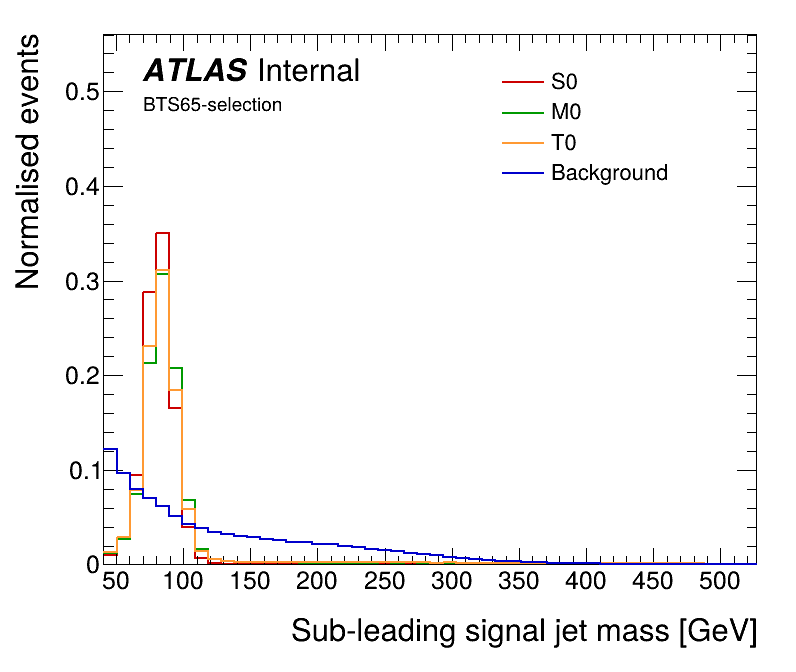
\includegraphics[width=\textwidth]{figures/SigJet2_M_NOSYS.png}
\end{subfigure}

\medskip

\begin{subfigure}[b]{0.4\textwidth}
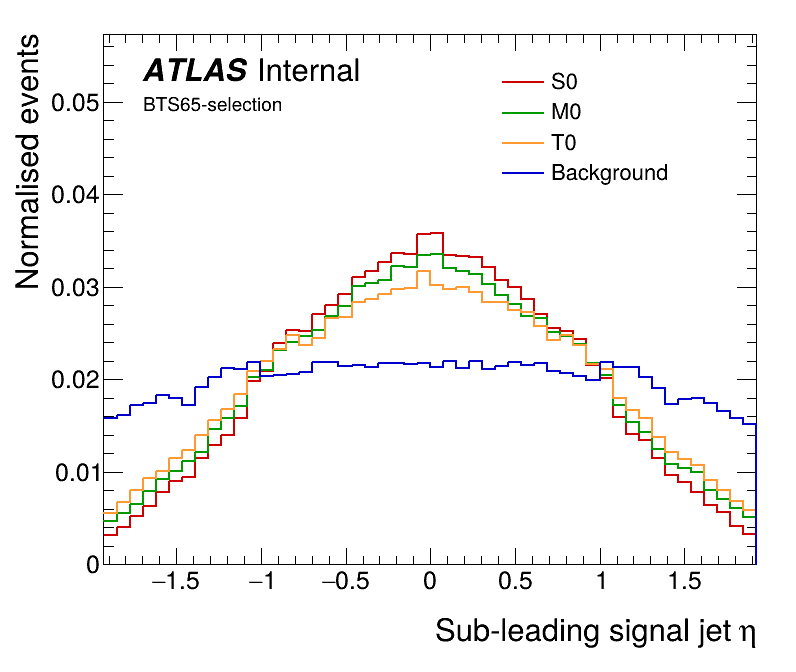
\includegraphics[width=\textwidth]{figures/SigJet2_eta_NOSYS.png}
\end{subfigure}
\hfill
\begin{subfigure}[b]{0.4\textwidth}
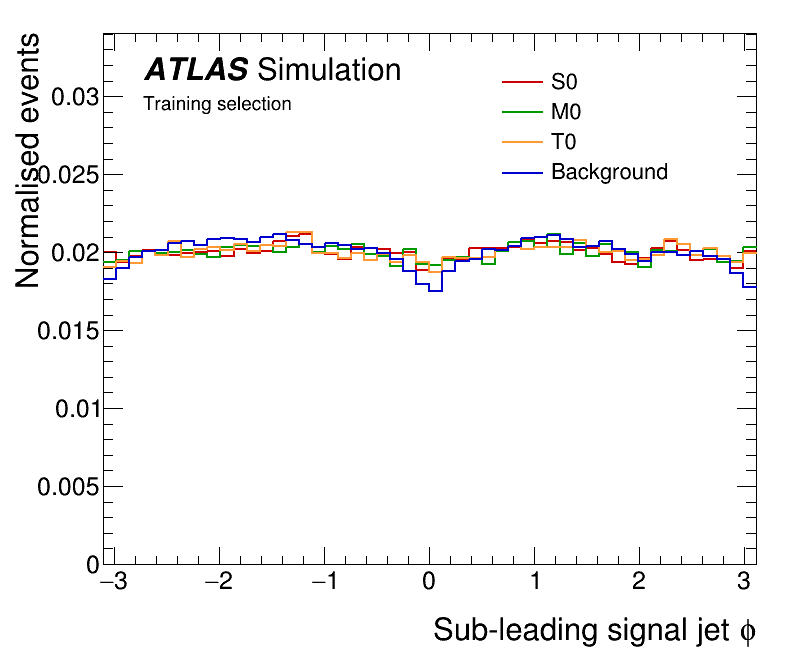
\includegraphics[width=\textwidth]{figures/SigJet2_phi_NOSYS.png}
\end{subfigure}
\caption{Normalised distributions of the eight kinematic MLP input features in the training selection. Top row (left to right): leading signal jet $p_T$, mass, $\eta$ and $\phi$. Bottom row: sub-leading signal jet $p_T$, mass, $\eta$ and $\phi$. Distributions are shown for representative S0 (red), M0 (green) and T0 (orange) aQGC signal samples and the composite background (blue). The signal jets are significantly harder and more central than the background and both jet masses peak near the $W/Z$ boson mass window for signal. The $\phi$ distributions are approximately uniform for all samples, as expected from the azimuthal symmetry of the detector.}
\label{fig:input_distributions}
\end{figure}

\begin{figure}[htbp]
\centering
\begin{subfigure}[b]{0.4\textwidth}
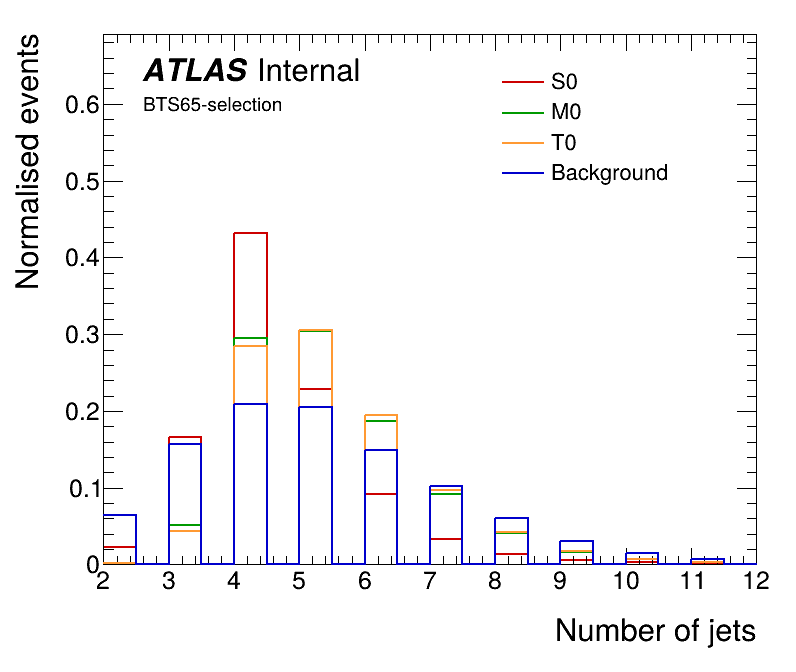
\includegraphics[width=\textwidth]{figures/nJets_NOSYS.png}
\end{subfigure}
\hfill
\begin{subfigure}[b]{0.4\textwidth}
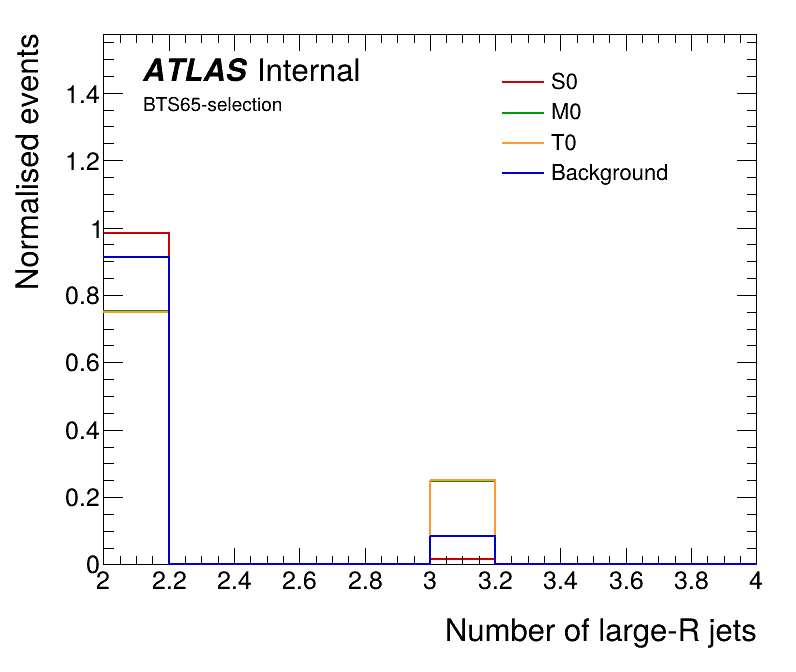
\includegraphics[width=\textwidth]{figures/nLargeRJets_NOSYS.png}
\end{subfigure}

\medskip

\begin{subfigure}[b]{0.4\textwidth}
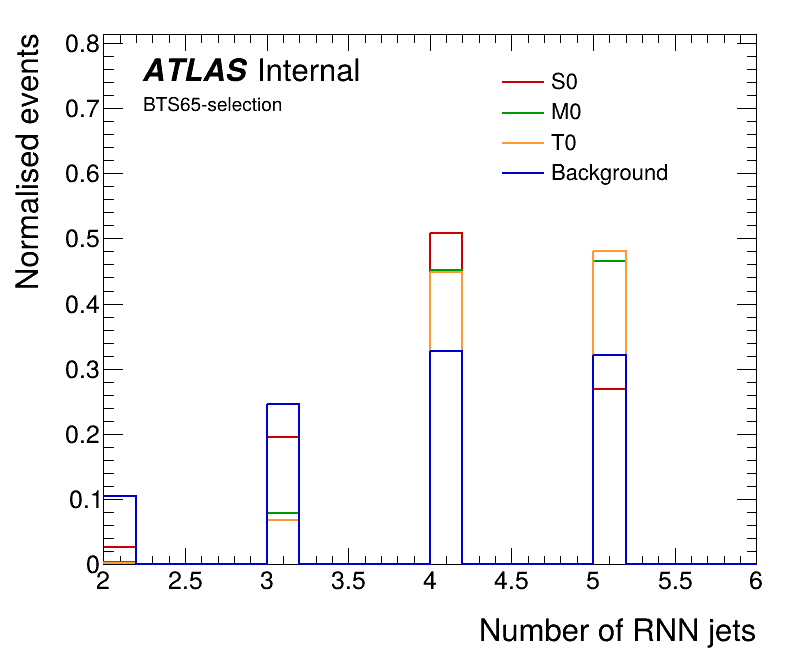
\includegraphics[width=\textwidth]{figures/nRNNJets_NOSYS.png}
\end{subfigure}
\hfill
\begin{subfigure}[b]{0.4\textwidth}
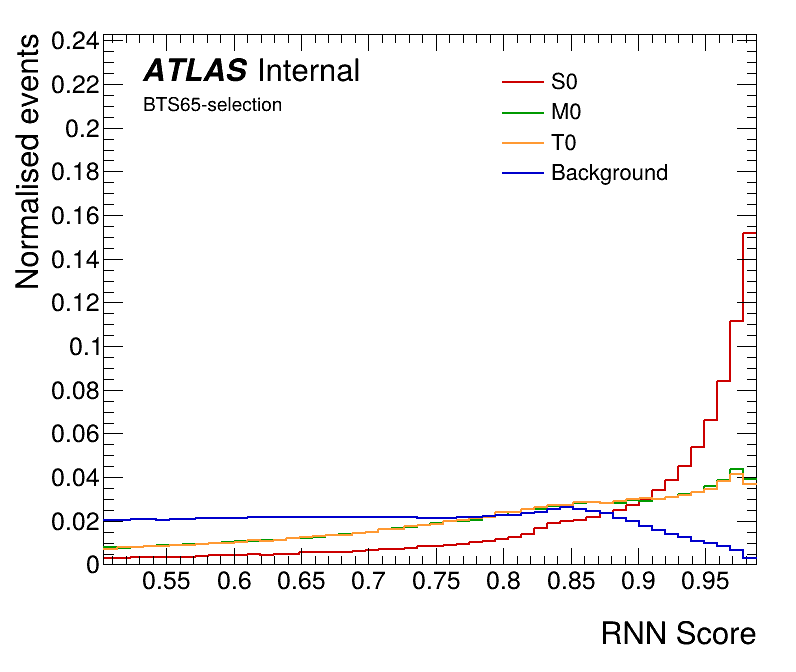
\includegraphics[width=\textwidth]{figures/RNNScore_NOSYS.png}
\end{subfigure}
\caption{Normalised distributions of the jet multiplicity and VBF-RNN input features in the training selection. Top row: total number of small-$R$ jets and number of large-$R$ jets, bottom row: number of RNN tagging jets and VBF-RNN v3 (6 jets) score. Distributions are shown for representative S0 (red), M0 (green) and T0 (orange) aQGC signal samples and the composite background (blue). Signal events tend to have higher jet multiplicities and are strongly peaked at high VBF-RNN scores, reflecting their characteristic VBS topology.}
\label{fig:input_distributions_extra}
\end{figure}

The background sample represents the full expected composition in the training selection, dominated by QCD dijet production ($\sim\!96\%$), with subdominant contributions from $V$+jets ($\sim\!3\%$), $t\bar{t}$ ($\sim\!1\%$), QCD diboson and electroweak $VV$+$jj$ production. Only the pure-EFT quadratic contribution to the signal cross section is used during training, as the linear interference term between the SM and EFT amplitudes is neglected in this analysis. To avoid the training being dominated by operators with large production cross sections, the aQGC signal samples are reweighted during training so that each operator contributes equally, effectively equalising their cross sections. The correct physical cross sections are restored when evaluating sensitivity.

\subsection{Binary classifier}

The binary classifier is an MLP with a single sigmoid output node, trained to assign a score $s \in [0,1]$ representing the probability that an event originates from aQGC signal. As discussed in Chapter~\ref{chap:ml}, the sigmoid activation together with the binary cross-entropy loss drives the network output towards the true posterior $P(y=1 \mid \mathbf{x})$.

Two variants of the binary classifier are trained. Specialised models are trained on a single operator family at a time, pairing the two lowest-index operators within each family: $\mathcal{O}_{S,0}+\mathcal{O}_{S,1}$, $\mathcal{O}_{M,0}+\mathcal{O}_{M,1}$, or $\mathcal{O}_{T,0}+\mathcal{O}_{T,1}$. A global model is trained on an ensemble of all available operators spanning the scalar, mixed and tensor families, $S(0\text{--}1) + M(0\text{--}5,\,7) + T(0\text{--}9)$, providing broad sensitivity across the full operator space without requiring a separate model for each operator.

\subsection{Multi-class classifier}

The binary approach assigns a single signal probability without distinguishing between operator families. Since the three operator families produce distinct kinematic signatures, as discussed in Chapter~\ref{chap:sm}, a natural extension is to train a single model that simultaneously identifies both the presence of aQGC signal and its operator family.

The multi-class classifier extends the output layer to $K=4$ nodes corresponding to background, scalar, mixed and tensor classes. A softmax activation is applied to produce a valid probability distribution $(\hat{y}_1,\dots,\hat{y}_K)$ over the four classes and the network is trained by minimising the categorical cross-entropy loss, following the multi-class formulation described in Chapter~\ref{chap:ml}. The network is trained on all available operators across all three families simultaneously, with class balancing applied to account for the differing numbers of operators per family.

\subsection{Architecture and training hyperparameters}

Both the binary and multi-class MLPs share a feed-forward architecture of fully connected hidden layers with ReLU activations, followed by an output layer whose form is dictated by the classification task: a single sigmoid node for the binary classifier and four softmax nodes for the multi-class classifier. The two networks differ in width, depth and dropout. The multi-class classifier is wider and uses slightly stronger dropout to control overfitting on the more granular labelling task, while the binary classifier is deeper but narrower. The complete set of architecture and training hyperparameters is given in Table~\ref{tab:mlp_hyperparams}.

\begin{table}[htbp]
  \centering
  \caption{Architecture and training hyperparameters of the binary and multi-class MLP discriminants. Both networks share fully connected hidden layers with ReLU activations and differ in the output layer dictated by the classification task, as well as in width, depth and dropout.}
  \label{tab:mlp_hyperparams}
  \begin{tabular}{|c|c|c|}
    \hline
    \textbf{Hyperparameter} & \textbf{Binary} & \textbf{Multi-class} \\
    \hline
    Width (hidden units per layer) & 64 & 128 \\
    Depth (hidden layers)          & 6  & 5 \\
    Dropout                        & 0.20 & 0.25 \\
    Hidden activation              & ReLU & ReLU \\
    Output activation              & Sigmoid & Softmax \\
    Output nodes                   & 1 & 4 \\
    Loss function                  & Binary cross-entropy & Categorical cross-entropy \\
    Input features                 & \multicolumn{2}{c|}{12 (Section~\ref{sec:mldiscriminant})} \\
    \hline
  \end{tabular}
\end{table}

\subsection{Final discriminant and significance estimation}

The final discriminant used for sensitivity estimation is the logarithm of the likelihood ratio derived from the classifier output. This transformation is motivated by the Neyman--Pearson lemma, which guarantees that the likelihood ratio is the most powerful test statistic for a simple hypothesis test; by training the classifier to approximate the posterior probabilities, the log-ratio of the outputs approximates the log-likelihood ratio and therefore approaches the optimal discriminant.

For the binary classifier, the single sigmoid output $p \in [0,1]$ encodes the signal posterior, so that $p_{\mathrm{signal}} = p$ and $p_{\mathrm{background}} = 1-p$. The discriminant reduces to the logit transformation of the output score,
\begin{equation}
D_{\mathrm{bin}} = \log\frac{p}{1-p}.
\end{equation}
For the multi-class classifier, the four softmax outputs $(p_b,p_S,p_M,p_T)$ provide separate estimates of the posterior probability for each class. A dedicated discriminant is constructed for every signal class $s \in \{S,M,T\}$ as
\begin{equation}
D_{\mathrm{mc}}^{(s)} = \log\frac{p_s}{p_b}, \qquad s \in \{S,M,T\},
\end{equation}
which is in general different from the binary logit since $p_b \neq 1 - p_s$ when the remaining two signal-class probabilities are non-zero. When evaluating sensitivity for an operator belonging to family $s$, the corresponding $D_{\mathrm{mc}}^{(s)}$ is used as the template variable. The resulting per-operator discriminant distributions and binned templates are shown in Section~\ref{sec:sens_discriminants}.

The discriminant is evaluated per individual operator across all model types and binned to form the final template used for sensitivity estimation. The binning is not fixed across models: for each operator and each discriminant, the bin edges are re-optimised such that every bin contains a minimum yield of three events in the least-populated background category. This requirement avoids regions of the template that are dominated by Monte Carlo statistical fluctuations of any single background process, which would otherwise bias the Asimov significance, while still allowing the high-score tail, where the signal-to-background ratio is largest, to be resolved as finely as the available background statistics permit.

The expected sensitivity is quantified using the Asimov binned significance with a per-bin Gaussian background uncertainty~\cite{Cowan:2010js}. The Asimov dataset is the single representative dataset in which every observed bin count is set equal to its expectation value under the tested hypothesis. Evaluating the profile-likelihood test statistic on this dataset yields the median expected significance without the need for pseudo-experiments. For a counting experiment with signal yield $s_i$, background yield $b_i$ and absolute background uncertainty $\sigma_{b,i}$ in bin $i$, the median discovery significance is
\begin{equation}
Z_A = \sqrt{\,2\sum_i\left[\,(s_i+b_i)\,\ln\!\frac{(s_i+b_i)\bigl(b_i+\sigma_{b,i}^{2}\bigr)}{b_i^{2}+(s_i+b_i)\sigma_{b,i}^{2}} \,-\,\frac{b_i^{2}}{\sigma_{b,i}^{2}}\ln\!\left(1+\frac{\sigma_{b,i}^{2}\,s_i}{b_i\bigl(b_i+\sigma_{b,i}^{2}\bigr)}\right)\right]}\,.
\label{eq:zasymptotic}
\end{equation}
A relative background normalisation uncertainty of $30\%$ is assumed throughout this work, so $\sigma_{b,i}=0.30\,b_i$ in every bin. The choice of $30\%$ is a conservative envelope of the per-process uncertainties on the QCD multijet, $V$+jets, $t\bar{t}$ and diboson backgrounds entering the training selection and is not yet replaced by a profile of the underlying nuisance parameters.

In the limit $\sigma_{b,i}\to 0$, Equation~\ref{eq:zasymptotic} reduces to the statistics-only Asimov form $Z_A=\sqrt{2\sum_i[(s_i+b_i)\ln(1+s_i/b_i)-s_i]}$, and the further limit $s_i\ll b_i$ recovers the Gaussian approximation $Z\approx s/\sqrt{b}$. In the analysis regime studied here, several high-score bins of the multivariate discriminants reach $s_i\sim b_i$ and the Gaussian approximation would overestimate the sensitivity. Equation~\ref{eq:zasymptotic} remains valid in that regime, since it is derived from the Poisson-times-Gaussian likelihood without assuming $s_i\ll b_i$, and is used throughout this thesis. To enable a direct comparison between operators with widely different production cross sections and between the various classifier architectures, results are presented normalised to the significance $Z_A^{m_{JJ}}$ obtained from a one-dimensional fit of the invariant mass $m_{JJ}$ of the two large-$R$ signal jets alone, computed with the same Equation~\ref{eq:zasymptotic}.